\documentclass[12pt]{article}
\usepackage{graphicx}
\usepackage{latexsym}
\usepackage{amssymb}
\usepackage[utf8]{inputenc}
\usepackage[T1]{fontenc}
\usepackage[french]{babel}
\usepackage[french,algoruled,vlined]{algorithm2e}
\usepackage{textcomp}
\usepackage{listings}
\usepackage{lstlinebgrd}
\definecolor{darkgreen}{rgb}{0, 0.6, 0}
\usepackage{multirow}
\usepackage{rotating}

\lstdefinelanguage[mips]{Assembler}%
{morestring=[b]",
morekeywords=[1]{abs,abs.d,abs.ps,abs.s,add,add.d,add.ps,add.s,addi,addiu,addu,alnv.ps,and,%
  andi,b,bal,bc1f,bc1fl,bc1t,bc1tl,bc2f,bc2fl,bc2t,bc2tl,beq,beql,beqz,bge,bgeu,bgez,%
  bgezal,bgezall,bgezl,bgt,bgtu,bgtz,bgtzl,ble,bleu,blez,blezl,blt,bltu,bltz,bltzal,%
  bltzall,bltzl,bne,bnel,bnez,break,c.eq.d,c.eq.ps,c.eq.s,c.f.d,c.f.ps,c.f.s,c.le.d,%
  c.le.ps,c.le.s,c.lt.d,c.lt.ps,c.lt.s,c.nge.d,c.nge.ps,c.nge.s,c.ngl.d,c.ngl.ps,%
  c.ngl.s,c.ngle.d,c.ngle.ps,c.ngle.s,c.ngt.d,c.ngt.ps,c.ngt.s,c.ole.d,c.ole.ps,c.ole.s,%
  c.olt.d,c.olt.ps,c.olt.s,c.seq.d,c.seq.ps,c.seq.s,c.sf.d,c.sf.ps,c.sf.s,c.ueq.d,c.ueq.ps,%
  c.ueq.s,c.ule.d,c.ule.ps,c.ule.s,c.ult.d,c.ult.ps,c.ult.s,c.un.d,c.un.ps,c.un.s,cache,%
  ceil.l.d,ceil.l.s,ceil.w.d,ceil.w.s,cfc0,cfc1,cfc2,clo,clz,cop2,ctc0,ctc1,ctc2,cvt.d.l,%
  cvt.d.s,cvt.d.w,cvt.l.d,cvt.l.s,cvt.ps.s,cvt.s.d,cvt.s.l,cvt.s.pl,cvt.s.pu,cvt.s.w,%
  cvt.w.d,cvt.w.s,deret,di,div,div.d,div.s,divu,ehb,ei,eret,ext,floor.l.d,floor.l.s,floor.w.d,%
  floor.w.s,ins,j,jal,jalr,jalr.hb,jr,jr.hb,l.d,l.s,la,lb,lbu,ld,ldc1,ldc2,ldxc1,lh,lhu,li,li.d,%
  li.s,ll,lui,luxc1,lw,lwc1,lwc2,lwl,lwr,lwxc1,madd,madd.d,madd.ps,madd.s,maddu,mfc0,mfc1,%
  mfc1.d,mfc2,mfhc1,mfhc2,mfhi,mflo,mov.d,mov.ps,mov.s,move,movf,movf.d,movf.ps,movf.s,movn,%
  movn.d,movn.ps,movn.s,movt,movt.d,movt.ps,movt.s,movz,movz.d,movz.ps,movz.s,msub,msub.d,msub.ps,%
  msub.s,msubu,mtc0,mtc1,mtc1.d,mtc2,mthc1,mthc2,mthi,mtlo,mul,mul.d,mul.ps,mul.s,mulo,%
  mulou,mult,multu,neg,neg.d,neg.ps,neg.s,negu,nmadd.d,nmadd.ps,nmadd.s,nmsub.d,nmsub.ps,%
  nmsub.s,nop,nor,not,or,ori,pll.ps,plu.ps,pref,prefx,pul.ps,puu.ps,rdhwr,rdpgpr,recip.d,%
  recip.s,rem,remu,rfe,rol,ror,rotr,rotrv,round.l.d,round.l.s,round.w.d,round.w.s,rsqrt.d,%
  rsqrt.s,s.d,s.s,sb,sc,sd,sdbbp,sdc1,sdc2,sdxc1,seb,seh,seq,sge,sgeu,sgt,sgtu,sh,sle,sleu,%
  sll,sllv,slt,slti,sltiu,sltu,sne,sqrt.d,sqrt.s,sra,srav,srl,srlv,ssnop,sub,sub.d,sub.ps,%
  sub.s,subu,suxc1,sw,swc1,swc2,swl,swr,swxc1,sync,synci,syscall,teq,teqi,tge,tgei,tgeiu,tgeu,%
  tlbp,tlbr,tlbwi,tlbwr,tlt,tlti,tltiu,tltu,tne,tnei,trunc.l.d,trunc.l.s,trunc.w.d,trunc.w.s,ulh,%
  ulhu,ulw,ush,usw,wrpgpr,wsbh,xor,xori},%
morekeywords=[2]{.alias,.align,.ascii,.asciiz,.asm0,.bgnb,.byte,.comm,.data,.double,.end,.endb,%
  .endr,.ent,.err,.extern,.file,.float,.fmask,.frame,.globl,.half,.kdata,.ktext,.lab,.lcomm,%
  .livereg,.loc,.mask,.noalias,.option,.rdata,.repeat,.sdata,.set,.space,.struct,.text,%
  .verstamp,.vreg,.word},%
comment=[l]\#%
}[keywords,comments,strings]

\lstset{
  upquote=true,
  columns=flexible,
  keepspaces=true,
  breaklines,
  breakindent=0pt,
  basicstyle=\ttfamily,
  breaklines=true,
  keywordstyle=\color{blue},
  commentstyle=\color{darkgreen},
  tabsize=2,
  escapechar={@},
  %        escapebegin=\color{gray},
  showspaces=false,
  showtabs=false,
  showstringspaces=true,
%  numbers=left
}


\setlength{\textheight}{240mm}
\setlength{\textwidth}{162mm}
\setlength{\topmargin}{-11mm}
\setlength{\oddsidemargin}{+1mm}
\setlength{\unitlength}{1cm}


\begin{document}
\noindent
{\bf Département d'informatique \hfill Architecture} \\
$3^{\grave{e}me}$ année
\vspace*{1cm}
\begin{center}
  {\large \bf Architecture \emph{MIPS} mono-cycle\\
    avec gestion des exceptions et des interruptions}
\end{center}

\renewcommand{\labelitemi}{$\bullet$}
\renewcommand{\labelitemii}{$\star$}

Nous allons ajouter à notre architecture sur un cycle la gestion des exceptions et des interruptions
et de nouvelles instructions.

\section{Modèle de programmation}

\subsection{Espace d'adressage}

Nous allons ajouter dans l'espace d'adressage de l'architecture mono-cycle un terminal qui sera géré par quatre
registres:

\begin{center}
  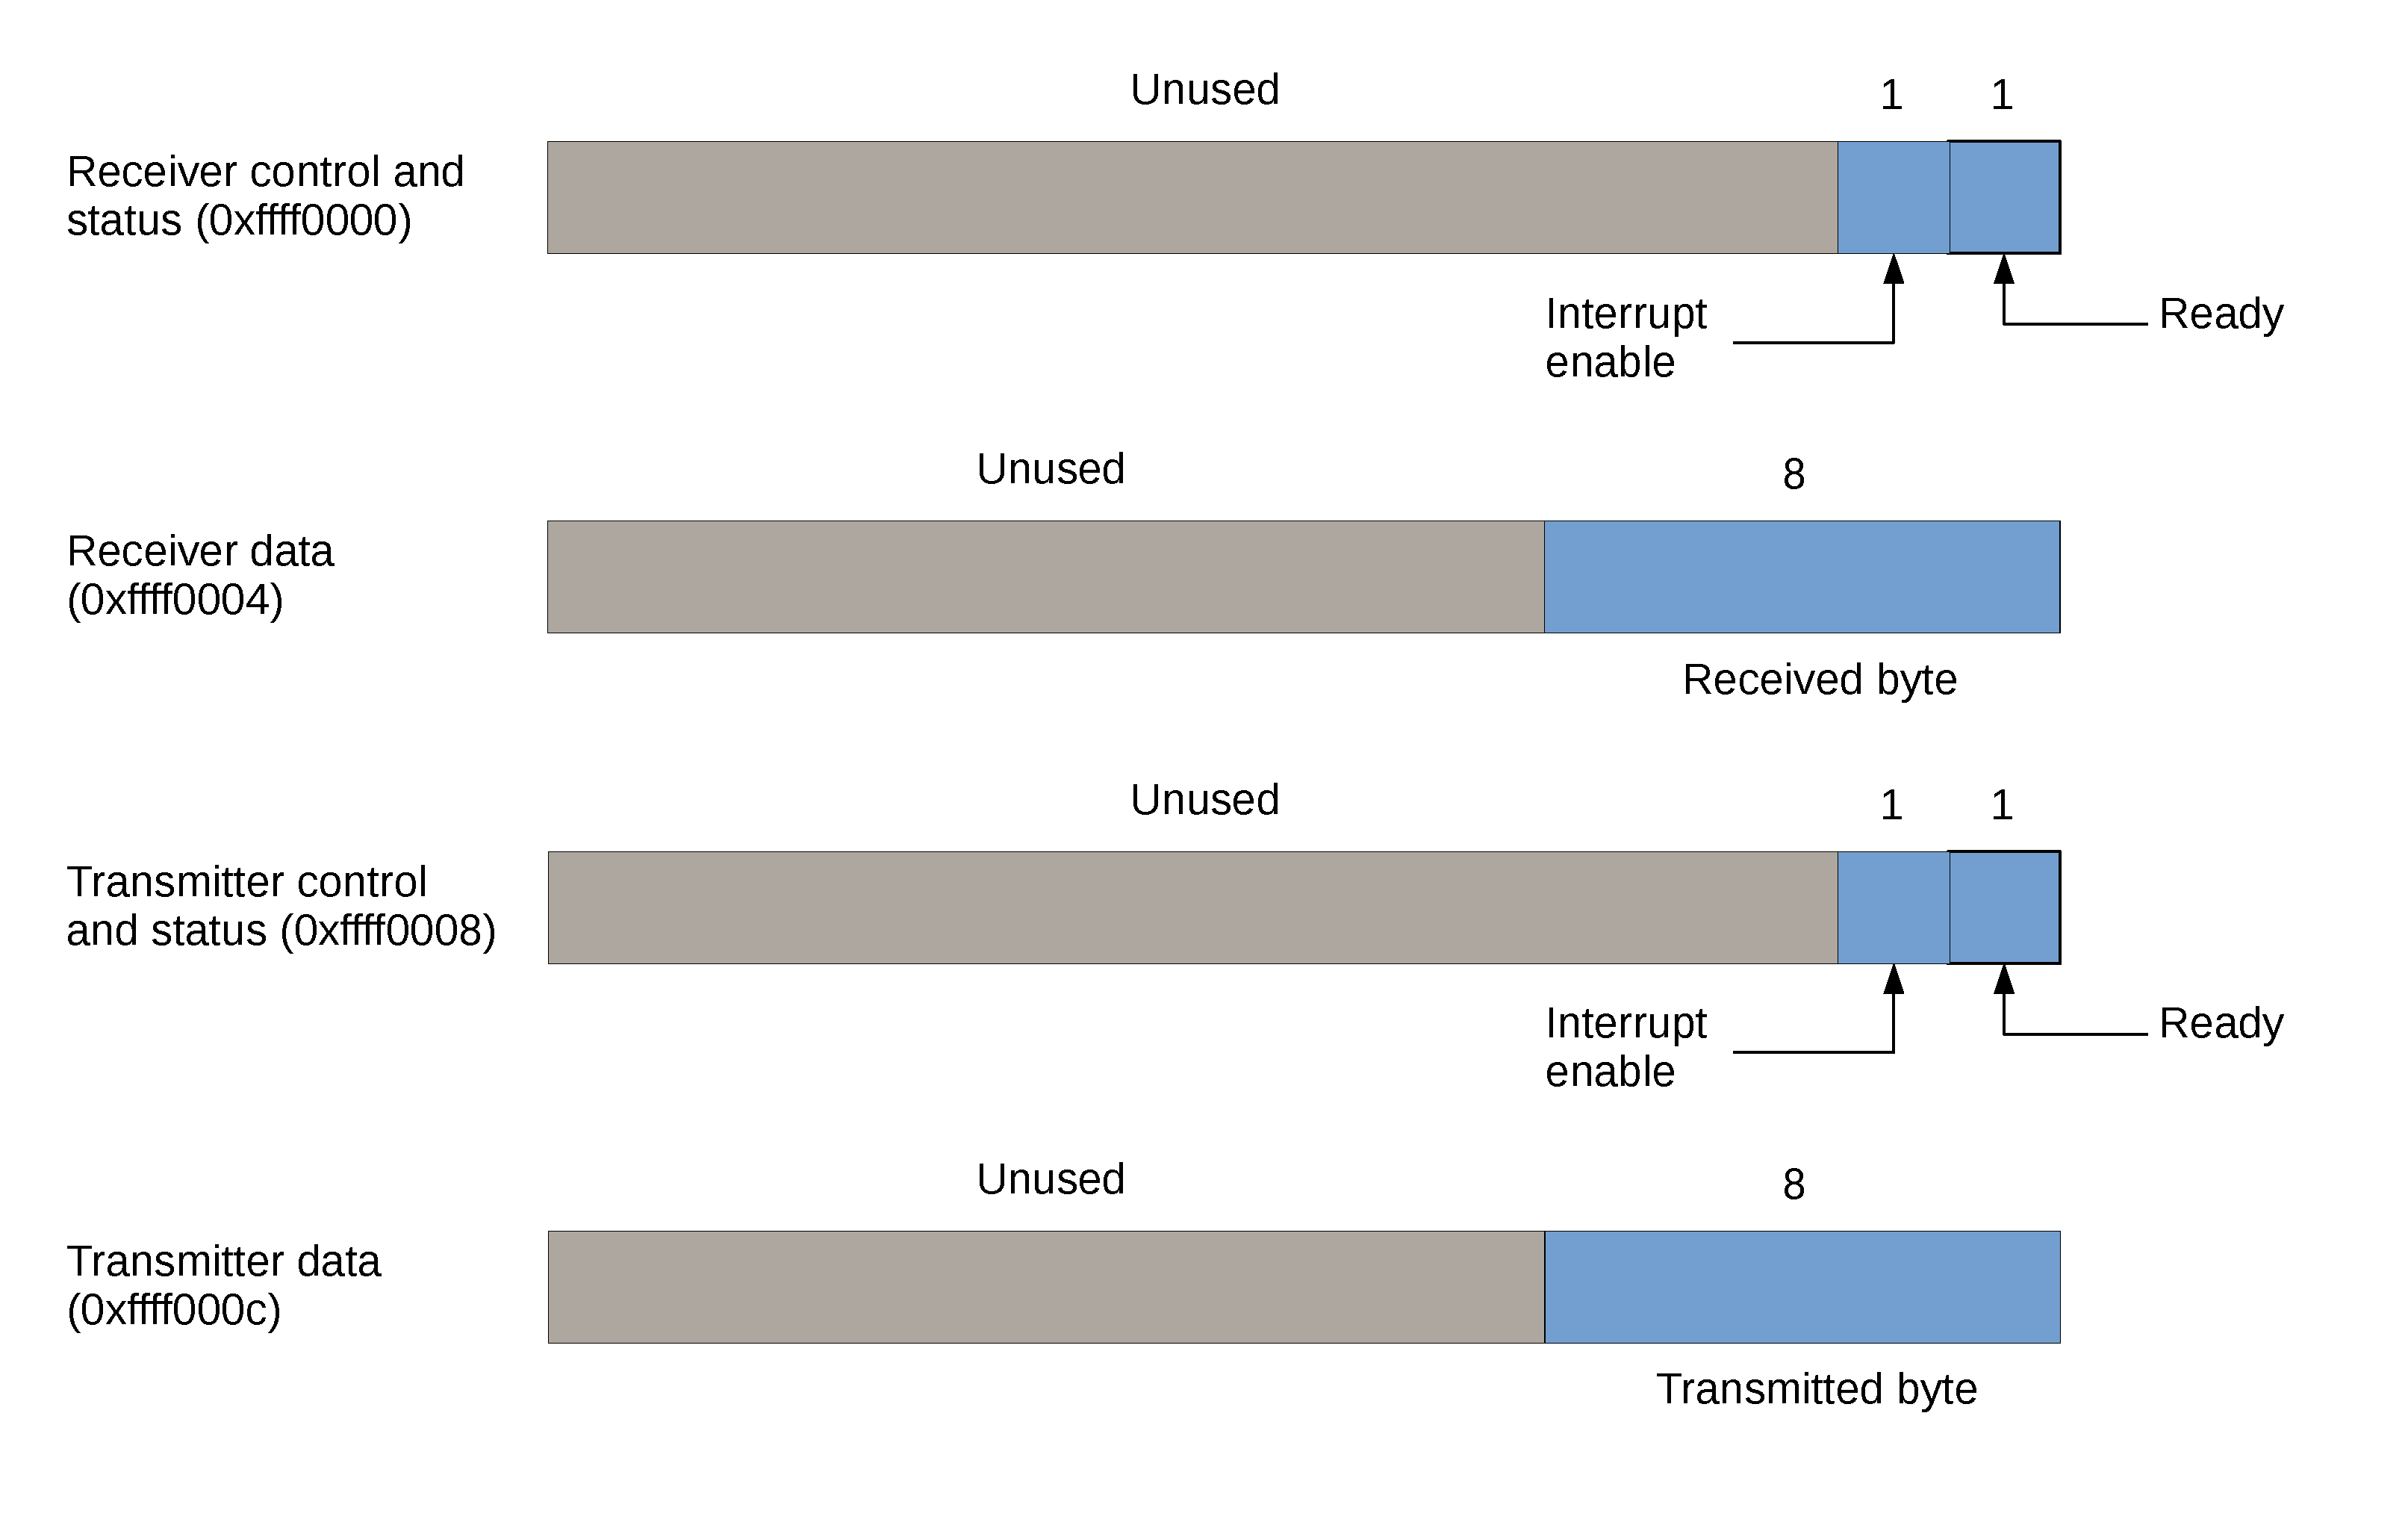
\includegraphics[width=18cm]{terminal.pdf}
\end{center}

Chacun de ces quatre registres, chacun sur $32$ bits, apparaissent comme quatre adresses mémoires particulières.\\

Le registre de contrôle et d'état en réception (\emph{Receiver control and status})
se trouve à l'adresse \verb+0xffff0000+. Si le bit \verb+0+ (\emph{Ready}) est à \verb+1+, cela signifie qu'un caractère est arrivé
depuis le clavier, mais qu'on a pas encore lu la donnée (\emph{Received byte}) du registre de donnée en réception (\emph{Receiver data}).
Si le bit \verb+1+ du registre de contrôle et d'état en réception (\emph{Interrupt enable}) est à $1$, une demande
d'interruption sera envoyée au processeur tant que le bit \emph{Ready} est à \verb+1+.
Lorsqu'on lit le registre de réception (\emph{Receiver data}), le bit \emph{Ready} passe à zéro. Initialement, les bits
\verb+Interrupt enable+ et \verb+Ready+ sont à $0$.\\

Le registre de contrôle et d'état en émission (\emph{Transmitter control and status}) se trouve à l'adresse \verb+0xffff0008+. Si le
bit \verb+0+ (\emph{Ready}) est à $1$, l'émetteur est prêt à recevoir un nouveau caractère. Si ce bit est à $0$, cela veut dire que l'émetteur
est toujours occupé à envoyer le précédent caractère. Si le bit \verb+1+ de ce registre est à $1$, une demande d'interruption sera envoyée au processeur
quand le bit \verb+0+ est à $1$, ce qui signifie que l'emetteur est prêt à envoyer un nouveau caractère. Le caractère que l'on veut envoyer est à écrire dans la
partie (\emph{Transmitted byte}) du registre d'émission (\emph{Transmitter data}). Initialement,
le bit \verb+Interrupt enable+ est à $0$ et le bit \verb+Ready+ est à $1$.\\

\subsection{Gestion des exceptions et des interruptions}

Nous allons implémenter de manière simplifiée la gestion des exceptions et des interruptions.
Dans la terminologie \emph{MIPS}, on parle d'interruption
pour un évènement extérieur au processeur (lié à un périphérique) et d'exception pour un évènement interne au processeur (division par zéro par exemple).\\

Dans notre implémentation,

\begin{itemize}

\item On ne gère que trois exceptions: débordement arithmétique, instruction non implémentée et appel système.

\item Les seules interruptions viennent du terminal.

\item On suppose que les instructions et exceptions sont masquées au lancement de la machine (registre \verb+Status+ à $0$).

\end{itemize}

\subsubsection{Registres}

L'architecture \emph{MIPS} possède normalement un coprocesseur $0$ pour gérer, entre autres, les exceptions et interruptions. Nous n'implémenterons
que trois des registres associés à ce coprocesseur : \verb+Status+, \verb+Cause+ et \verb+EPC+.

\begin{itemize}

\item Le registre numéro $12$, appelé \emph{Status register} (pour registre d'état), permet de savoir si les exceptions ou les interruptions
  sont masquées ou non. Ce registre est décrit ci-dessous~:\\

\begin{center}
\begin{tabular}{ccrrrr}
 & & \begin{sideways} Overflow \end{sideways} & \begin{sideways} Unimplemented \end{sideways} & \begin{sideways} Syscall \end{sideways} & \begin{sideways} Int \end{sideways}\\
 31 : 8 & 7 : 4 & 3 & 2 & 1 & 0\\
\hline
\multicolumn{1}{|c}{\hspace*{3cm}Unused\hspace*{3cm}} & \multicolumn{1}{|c|}{\hspace*{1cm}Save\hspace*{1cm}} & \multicolumn{1}{|c|}{} & \multicolumn{1}{|c|}{} & \multicolumn{1}{|c|}{} & \multicolumn{1}{|c|}{} \\
\hline
\end{tabular}
\end{center}

\vspace{0.7cm}

La signification des différents champs est la suivante~:
\begin{itemize}
\item Le bit \verb+0+ est à $0$ si les demandes d'interruptions (arrivant sur la broche \verb+Int+ du processeur) sont masquées. Elle est à $1$
sinon.
\item Le bit \verb+1+ est à $0$ si les appels systèmes sont masqués. Elle est à $1$
sinon.
\item Le bit \verb+2+ est à $0$ si l'exception correspondant à une instruction non implémentée est masquée. Elle est à $1$
sinon.
\item Le bit \verb+3+ est à $0$ si l'exception correspondant à un débordement est masquée. Elle est à $1$
sinon.
\item Les bits \verb+4+ à \verb+7+ permettent de sauvegarder les quatre premiers bits lors du traitement d'une interruption ou d'une exception.\\
\end{itemize}



\item Le registre numéro $13$, appelé \emph{Cause register} (pour registre de cause), permet de connaître la cause d'une exception ou d'une interruption.
Ce registre est décrit ci-dessous~:\\

\begin{center}
\begin{tabular}{ccc}
 31 : 2 & 1 : 0\\
\hline
\multicolumn{1}{|c}{\hspace*{5cm}Unused\hspace*{5cm}} & \multicolumn{1}{|c|}{ExcCode}\\
\hline
\end{tabular}
\end{center}

\vspace{0.7cm}

Les bits \verb+0+ et \verb+1+ contiennent un nombre indiquant le type d'exception ou d'interruption qui vient de se produire. Les différentes valeurs
qui nous intéressent sont décrites dans la table \ref{table:int}.\\

\begin{table}[!htpb]
\begin{center}
\begin{tabular}{|c|c|p{7cm}|}
\hline
Valeur du champ \verb+Exception Code+ & Nom & Description\\
\hline
\hline
$0$ & \verb+Int+ & Interruption provenant d'un contrôleur de périphérique\\
\hline
$1$ & \verb+Syscall+ & On vient d'exécuter l'instruction \verb+syscall+\\
\hline
$2$ & \verb+Unimplemented+ & L'instruction n'est pas valide (instruction non reconnue)\\
\hline
$3$ & \verb+Overflow+ & Un débordement s'est produit pour une instruction arithmétique\\
\hline
\end{tabular}
\end{center}
\caption{Les différentes valeurs du champ \emph{Exception Code}.}
\label{table:int}
\end{table}

\vspace{0.5cm}

\item Le registre numéro $14$, appelé \verb+EPC+, permet de sauvegarder la valeur du compteur ordinal (\verb+PC+) lors de la prise en compte
d'une exception ou d'une interruption.

\end{itemize}

\subsubsection{Déroulement de la gestion d'une exception ou d'une interruption}

Notre gestion simplifiée des interruptions et des exceptions est la suivante :

\begin{itemize}

\item Pour les exceptions, l'adresse de l'instruction qui a déclenchée
  celle-ci est sauvegardée dans le registre \verb+EPC+. Pour les interruptions,
  l'adresse de l'instruction suivante est sauvegardée dans \verb+EPC+.

\item Le contenu du registre \verb+Status+ est décalé à gauche de $4$ bits afin de sauvegarder
  les valeurs actuelles de ce registre et de masquer les interruptions et les exceptions.

\item Le champ \verb+ExcCode+ du registre \verb+Cause+ est mis à jour.

\item On met dans le compeur ordinal l'adresse \verb+0x80000180+ qui est celle du traitant d'interruption.

\item Lorsque l'on sort du traitant d'interruption ou d'exception (instruction \verb+eret+), le contenu du registre \verb+Status+
  est restauré en le décalant de $4$ bits vers la droite.

\item On remet dans le compteur ordinal la valeur de \verb+EPC+.

\end{itemize}

\subsubsection{Instructions}

Nous allons ajouter quatre nouvelles instructions qui vont permettre de réaliser des appels système dans le cadre des systèmes d'exploitation (\verb+syscall+),
de sortir d'un traitant d'interruption (\verb+eret+), de déplacer des valeurs du banc de registres du processeur vers celui du coprocesseur $0$ (\verb+mtc0+)
et de déplacer des valeurs du banc de registres du coprocesseur $0$ vers celui du processeur (\verb+mfc0+).\\

\begin{itemize}
\item \verb+syscall+\\
Cette instruction permet de générer une exception afin de passer la main au système
d'exploitation. L'addresse de l'instruction est sauvegardée dans le registre \verb+EPC+, la cause de l'exception \verb+Syscall+ est
placée dans le registre de cause (\emph{Cause register}) (voir la table \ref{table:int}).
Le compteur ordinal est alors chargé avec l'adresse du traitant
d'exceptions ou d'interruptions (adresse \verb+0x80000180+).
L'instruction \verb+syscall+ est codée en langage machine~:\\
\begin{center}
\begin{tabular}{cc}
\hline
\multicolumn{1}{|c}{0} & \multicolumn{1}{|c|}{001100}\\
\hline
$26$ bits & $6$ bits\\
&\\
\end{tabular}
\end{center}

\item \verb+eret+\\
Cette instruction permet de sortir d'un traitant d'exceptions ou d'interruptions. Elle a pour effet de remettre simultanément le compteur ordinal à la valeur sauvegardée
dans le registre \verb+EPC+ et de décaler de $4$ vers la droite le registre \verb+Status+.
L'instruction \verb+eret+ est codée en langage machine~:\\
\begin{center}
\begin{tabular}{cccc}
\hline
\multicolumn{1}{|c}{100000} & \multicolumn{1}{|c}{1} & \multicolumn{1}{|c}{0} & \multicolumn{1}{|c|}{011000}\\
\hline
$6$ bits & $1$ bits & $19$ bits & $6$ bits\\
&&&\\
\end{tabular}
\end{center}

\item \verb+mtc0 rt, rd+\\
Cette instruction permet de copier la valeur du registre numéro \verb+rt+ du banc de registres du processeur vers le registre
numéro \verb+rd+ du banc de registres du coprocesseur $0$.
L'instruction \verb+mtc0 rt, rd+ est codée en langage machine~:\\
\begin{center}
\begin{tabular}{ccccc}
\hline
\multicolumn{1}{|c}{010000} & \multicolumn{1}{|c}{00100} & \multicolumn{1}{|c}{rt} & \multicolumn{1}{|c}{rd} & \multicolumn{1}{|c|}{0} \\
\hline
$6$ bits & $5$ bits & $5$ bits & $5$ bits & $11$ bits\\
&&&&\\
\end{tabular}
\end{center}

\item \verb+mfc0 rd, rt+\\
Cette instruction permet de copier la valeur du registre numéro \verb+rt+ du banc de registres du coprocesseur $0$ vers le registre
numéro \verb+rd+ du banc de registres du processeur.
L'instruction \verb+mfc0 rd, rt+ est codée en langage machine~:\\
\begin{center}
\begin{tabular}{ccccc}
\hline
\multicolumn{1}{|c}{010000} & \multicolumn{1}{|c}{0} & \multicolumn{1}{|c}{rt} & \multicolumn{1}{|c}{rd} & \multicolumn{1}{|c|}{0} \\
\hline
$6$ bits & $5$ bits & $5$ bits & $5$ bits & $11$ bits\\
&&&&\\
\end{tabular}
\end{center}

\end{itemize}

\subsection{Jeu complet d'instructions}

Le jeu complet d'instructions de notre architecture \emph{MIPS} est décrit dans la table \ref{table:instructions}.

\begin{table}[!htpb]
\begin{center}
\begin{tabular}{|l|c|c|c|c|c|c|l|}
  \hline
  \multicolumn{1}{|c|}{Inst.} & $[31:26]$ & $[25:21]$ & $[20:16]$ & $[15:11]$ & $[10:6]$ & $[5:0]$ & \multicolumn{1}{|c|}{Signification}\\
  \hline
  \hline
  \textbf{add} & 000000 & rs & rt & rd & 00000 & 100000 & R[rd] $\leftarrow$ R[rs] $+$ R[rt]\\
  \hline
  \textbf{sub} & 000000 & rs & rt & rd & 00000 & 100010 & R[rd] $\leftarrow$ R[rs] $-$ R[rt]\\
  \hline
  \textbf{and} & 000000 & rs & rt & rd & 00000 & 100100 & R[rd] $\leftarrow$ R[rs] \verb+&+ R[rt]\\
  \hline
  \textbf{or} & 000000 & rs & rt & rd & 00000 & 100101 & R[rd] $\leftarrow$ R[rs] \verb+|+ R[rt]\\
  \hline
  \textbf{xor} & 000000 & rs & rt & rd & 00000 & 100110 & R[rd] $\leftarrow$ R[rs] \verb+^+ R[rt]\\
  \hline
  \multirow{2}{*}{\textbf{slt}} & \multirow{2}{*}{000000} & \multirow{2}{*}{rs} & \multirow{2}{*}{rt} & \multirow{2}{*}{rd}
  & \multirow{2}{*}{00000} & \multirow{2}{*}{101010} & R[rd] $\leftarrow$ 1 si R[rs] $<$ R[rt]\\
                                                   & & & & & & & R[rd] $\leftarrow$ 0 sinon\\
  \hline
  \textbf{sll} & 000000 & 00000 & rt & rd & sa & 000000 & rd $\leftarrow$ rs \verb+<<+ sa\\
  \hline
  \textbf{srl} & 000000 & 00000 & rt & rd & sa & 000010 & rd $\leftarrow$ rs \verb+>>>+ sa\\
  \hline
  \textbf{sra} & 000000 & 00000 & rt & rd & sa & 000011 & rd $\leftarrow$ rs \verb+>>+ sa\\
  \hline
  \textbf{addi} & 001000 & rs & rt & \multicolumn{3}{|c|}{v(aleur immédiate)} & R[rt] $\leftarrow$ R[rs] + (signe)v\\
  \hline
  \textbf{andi} & 001100 & rs & rt & \multicolumn{3}{|c|}{v(aleur immédiate)} & R[rt] $\leftarrow$ R[rs] \verb+&+ (zéro)v\\
  \hline
  \textbf{ori} & 001101 & rs & rt & \multicolumn{3}{|c|}{v(aleur immédiate)} & R[rt] $\leftarrow$ R[rs] \verb+|+ (zéro)v\\
  \hline
  \textbf{xori} & 001110 & rs & rt & \multicolumn{3}{|c|}{v(aleur immédiate)} & R[rt] $\leftarrow$ R[rs] \verb+^+ (zéro)v\\
  \hline
  \textbf{lui} & 001111 & 00000 & rt & \multicolumn{3}{|c|}{v(aleur immédiate)} & R[rt] $\leftarrow$ v \verb+<<+ 16\\
  \hline
  \textbf{lw} & 100011 & rs & rt & \multicolumn{3}{|c|}{d(éplacement)} & R[rt] $\leftarrow$ M[R[rs] + (signe)d]\\
  \hline
  \textbf{sw} & 101011 & rs & rt & \multicolumn{3}{|c|}{d(éplacement)} & M[R[rs] + (signe)d] $\leftarrow$ R[rt]\\
  \hline
  \multirow{2}{*}{\textbf{beq}} & \multirow{2}{*}{000100} & \multirow{2}{*}{rs} & \multirow{2}{*}{rt} & \multicolumn{3}{|c|}{\multirow{2}{*}{d(éplacement)}} & si R[rs] $=$ R[rt] alors\\
      &        &    &    & \multicolumn{3}{|c|}{} & \ \ pc $\leftarrow$ pc + 4 + d * 4\\
  \hline
  \multirow{2}{*}{\textbf{bne}} & \multirow{2}{*}{000101} & \multirow{2}{*}{rs} & \multirow{2}{*}{rt} & \multicolumn{3}{|c|}{\multirow{2}{*}{d(éplacement)}} & si R[rs] $\ne$ R[rt] alors\\
      &        &    &    & \multicolumn{3}{|c|}{} & \ \ pc $\leftarrow$ pc + 4 + d * 4\\
  \hline
  \textbf{j} & 000010 & \multicolumn{5}{|c|}{a(dresse)} & pc $\leftarrow$ (pc + 4)$_{[31:28]}$(a * 4)$_{[27:0]}$\\
  \hline
  \multirow{2}{*}{\textbf{jal}} & \multirow{2}{*}{000011} & \multicolumn{5}{|c|}{\multirow{2}{*}{a(dresse)}} & R[\$31] $\leftarrow$ pc + 4\\
                       &                         & \multicolumn{5}{|c|}{}                           & pc $\leftarrow$ (pc + 4)$_{[31:28]}$(a * 4)$_{[27:0]}$\\
  \hline
  \textbf{jr} & 000000 & rs & 00000 & 00000 & 00000 & 001000 & pc $\leftarrow$ R[rs]\\
  \hline
  \textbf{mfc0} & 010000 & 00000 & rt & rd & 00000 & 000000 & R[rd] $\leftarrow$ C0\_R[rt]\\
  \hline
  \textbf{mtc0} & 010000 & 00100 & rt & rd & 00000 & 000000 & C0\_R[rd] $\leftarrow$ R[rt]\\
  \hline
  \textbf{syscall} & 000000 & 00000 & 00000 & 00000 & 00000 & 011000 & appel système\\
  \hline
  \multirow{2}{*}{\textbf{eret}} & \multirow{2}{*}{000000} & \multirow{2}{*}{00000} &
  \multirow{2}{*}{00000} & \multirow{2}{*}{00000} & \multirow{2}{*}{00000} & \multirow{2}{*}{011000} & retour du traitant d'exception\\
  & & & & & & & ou d'interruption\\
  \hline
\end{tabular}
\end{center}
\caption{Notre jeu complet d'instructions pour notre implémentation de \emph{MIPS}.}
\label{table:instructions}
\end{table}

On pourra aussi utiliser la pseudo-instruction \verb+la+, qui permet de charger l'adresse d'un label dans un registre. Par exemple, le programme suivant,\\
\begin{tabular}{c}
\begin{lstlisting}
  .bss
  input_index:  .word
  .text
  la $t0, input_index

\end{lstlisting}
\end{tabular}

mettra l'adresse du label \verb+input_index+ dans le registre \verb+$t0+.\\

On pourra aussi utiliser la pseudo-instruction \verb+li+ qui permet de charger une valeur sur $32$ bits dans un registre, par exemple,
\lstinline+li $t0, 0xbadcaffe+.


\subsection{Programmation de la gestion du terminal}

Nous supposons que nous disposons de toutes les instructions de la table \ref{table:instructions}. Notons que les registres \verb+$k0+ et \verb+$k1+
sont réservés pour le système d'exploitation et pourront être utilisés sans avoir à être sauvegardés dans le traitant d'exceptions et d'interruptions.

\subsubsection{Réception par attente active}

\'Ecrire la fonction \verb+read_busy_waiting+ permettant de stocker, en utilisant de l'attente active, les éléments reçus du clavier dans le buffer
\verb+input_buffer+. On suppose, pour simplier, que le buffer ne sera jamais plein.\\

\lstset{language=[mips]Assembler}

\begin{tabular}{c}
\begin{lstlisting}
  .kdata
input_index:  .word 0
input_buffer: .space BIG

  .ktext
read_busy_waiting:
  # to do
\end{lstlisting}
\end{tabular}

\subsubsection{Réception par interruption}

\'Ecrire le traitant d'interruption, \verb+it_handler+, qui permet de stocker les éléments reçus du clavier dans le buffer \verb+input_buffer+.\\

\begin{tabular}{c}
\begin{lstlisting}
  .kdata
input_index:  .word 0
input_buffer: .space BIG

  .ktext 0x80000180
it_handler:
  # to do
\end{lstlisting}
\end{tabular}

\subsubsection{\'Emission par attente active}

\'Ecrire la fonction \verb+write_busy_waiting+ permettant d'écrire, en utilisant de l'attente active, les éléments du buffer
\verb+output_buffer+ vers le terminal. Pour simplifier, on suppose que le buffer contient une quantité énorme de données, et on ne se
soucie pas de savoir quand on a atteint la fin de celui-ci.\\

\lstset{language=[mips]Assembler}

\begin{tabular}{c}
\begin{lstlisting}
  .kdata
output_index:  .word 0
output_buffer: .space BIG

  .ktext
write_busy_waiting:
  # to do
\end{lstlisting}
\end{tabular}

\subsubsection{\'Emission par interruption}

\'Ecrire le traitant d'interruption, \verb+it_handler+, qui permet d'envoyer les éléments du buffer \verb+output_buffer+ vers le terminal.\\

\lstset{language=[mips]Assembler}

\begin{tabular}{c}
\begin{lstlisting}
  .kdata
output_index:  .word 0
output_buffer: .space BIG

  .ktext 0x80000180
it_handler:
  # to do
\end{lstlisting}
\end{tabular}

\subsection{Modification de l'architecture mono-cycle}

Nous rappelons ici l'architecture réalisée lors du dernier TD :
\begin{itemize}
\item La figure \ref{fig:mips_datapath} décrit l'unité de traitement.
\item La table \ref{table:mips_control} décrit l'unité de contrôle.\\
\end{itemize}

\begin{figure}[!htpb]
\begin{center}
  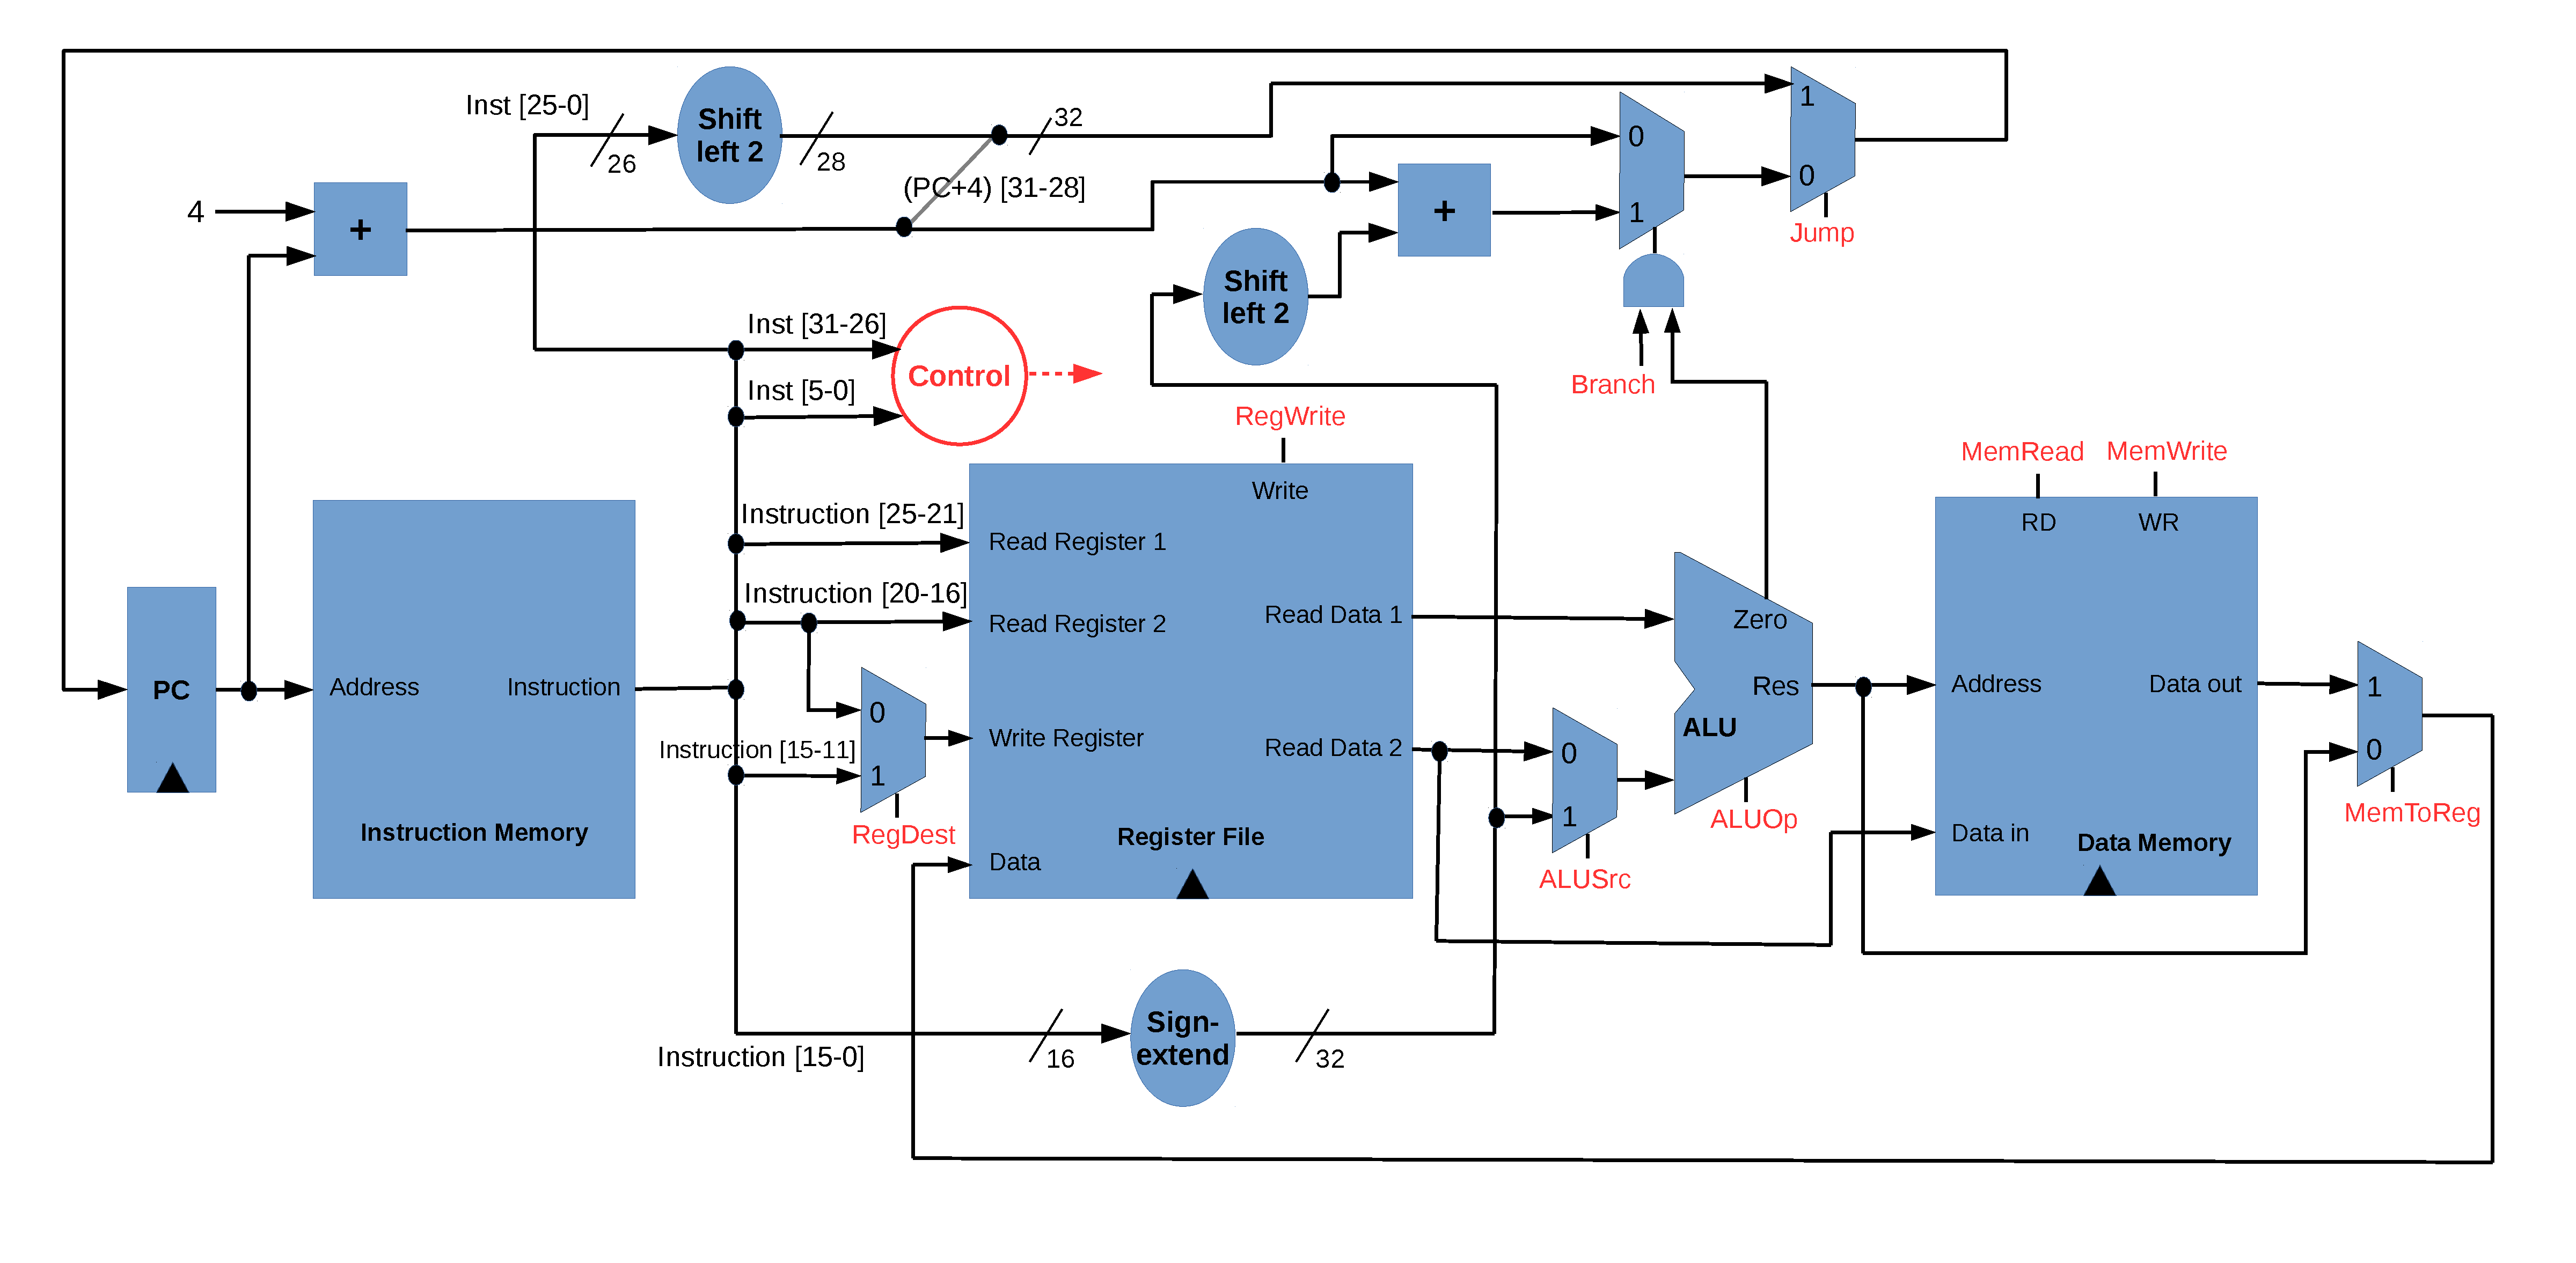
\includegraphics[width=19cm]{complete_single_cycle.pdf}
\end{center}
\caption{Unité de traitement de l'architecture mono-cycle.}
\label{fig:mips_datapath}
\end{figure}

\begin{table}[!htpb]
\begin{center}
\begin{tabular}{|c|c|}
\hline
Ligne de contrôle & Condition\\
\hline
\hline
\verb+RegDst+ & op = 0\\
\hline
\verb+RegWrite+ & op = 0 ou op = lw\\
\hline
\verb+ALUSrc+ & op = lw ou op = sw\\
\hline
\verb+Branch+ & op = beq\\
\hline
\verb+Jump+ & op = j\\
\hline
\verb+MemRead+ & op = lw\\
\hline
\verb+MemWrite+ & op = sw\\
\hline
\verb+MemToReg+ & op = lw\\
\hline
\verb+ALUOp0+ & op = beq\\
\hline
\verb+ALUOp1+ & op = 0\\
\hline
\end{tabular}
\end{center}
\caption{Contrôle de l'architecture mono-cycle.}
\label{table:mips_control}
\end{table}

Ajouter la gestion des exceptions et des interruptions à l'architecture mono-cycle.

%%\section{Architecture complète}


%% \subsection{Unité de traitement}

%% \subsection{Unité de contrôle}

%% \subsubsection{Contrôle de l'unité arithmétique et logique}

%% \subsubsection{Contrôle principal}

\end{document}
